\section{Problem description} \label{sec:problem}
During pipelay every few minutes a new pipe (new joint) section must be fitted onto the end of the existing pipeline (main line).
For decades in the offshore industry this has been a manual process. Allseas is working on a method to automate this.

\subsection{Main requirements for automated line-up}
Several projects have been initiated to automate the line-up process starting as early as 2008. However, These have all been
unsuccessful. The latest project was started in 2017 and is still ongoing. The main requirements are:
\begin{enumerate}
      \item Reducing line-up cycle times in the beadstall; This will result in significant cost reduction by
            decreasing vessel production time.
      \item Increasing accuracy of line-ups (reduce amount of root pass weld errors); This will also reduce
            costs due to decreasing vessel production time.
      \item Providing a safer work environment for the people working in the beadstall.
\end{enumerate}

\subsection{Current situation}
The latest iteration of automated line-up is a system that uses 5 laser line scanners to measure the pipe ends' position and orientation
(see figure \ref{fig:portal}).
\begin{figure}[H]
      \centering
      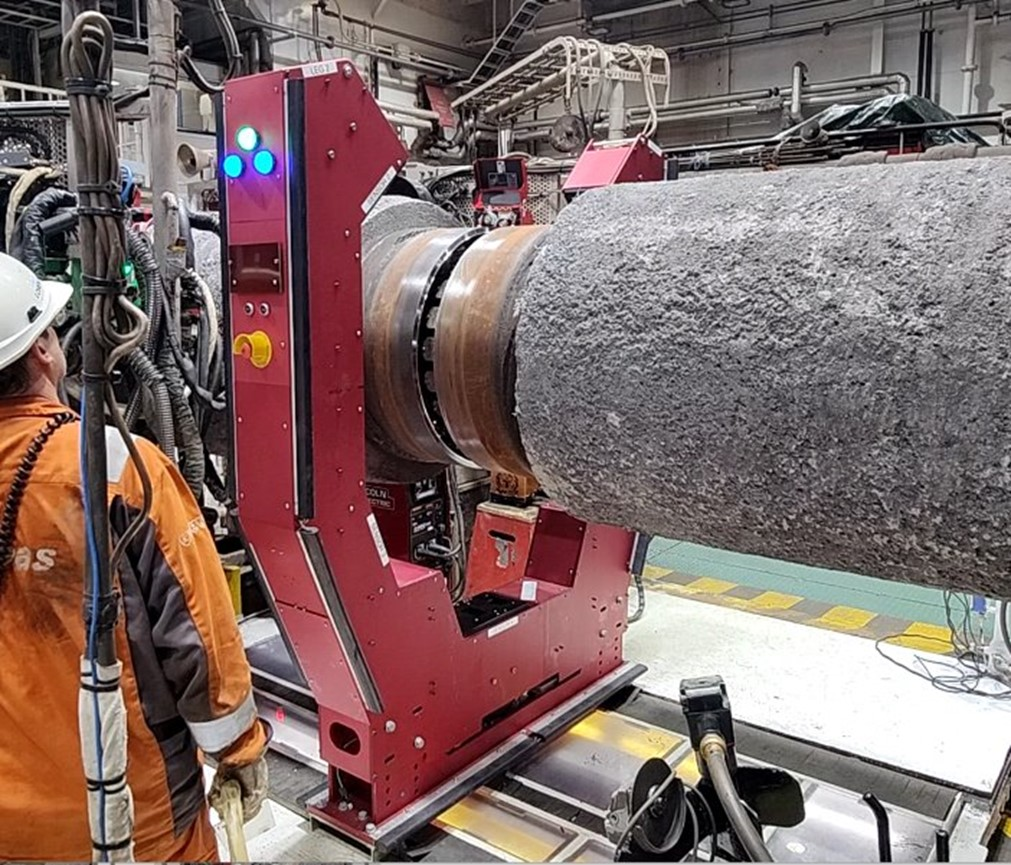
\includegraphics[width=0.7\textwidth]{images/side_view_final_lineup.jpg}
      \caption{The portal or `U-Frame'. The mainline is held in place in the background,
            while the new joint is lined up using instructions from automated line-up.
            The white stickers on the side of the frame indicate the position of the laser line scanners.
            Three on the side from which the picture is taken and two on the other side of the pipe.
            The U-Frame is mounted on the interface frame, which in turn is connected to the subframe.
            The subframe has motorized rollers and linear guides that allow the U-Frame to move with the new joint.
            This way the U-Frame ensures optimal visibility of the pipe ends for the laser line scanners. Additionally,
            the U-Frame can be moved out of way of other equipment, personel or operations when not in use.}
      \label{fig:portal}
\end{figure}

The laser line scanners generate 4192 data points in 5 different planes with a frequency of 60 $\sim$ 70 Hz. Initially,
a line finding algorithm derived from a Hough transform \cite{hough_transform} is used to recover approximately
straight sections from the laser's projection on the pipe. This allows for the recognition of the pipe ends or `bevels'
from the data.

Subsequently, the found pipe ends of the 5 sensors are combined to form a 3D representation of the pipe face.
This is done using using a combination of Newton-Raphson optimization and a least squares fit.

\subsection{Internship goals} \label{ssec:intern_goals}
The internship aims to improve the current automated line-up system by:
\begin{enumerate}
      \item [\textbf{a}] \textbf{Decreasing code execution time} by searching for and replacing
      slow or redundant operations;
      \item [\textbf{b}] \textbf{Writing maintainable code} by refactoring the current codebase;
      \item [\textbf{c}] \textbf{Increasing machine accuracy} by comparing different pipe fitting algorithms.
\end{enumerate}
